\section{更新方法(初次安装使用可跳过)}

\textbf{\color{red}\lstinline{lua} 目录下的 \lstinline{Setting.lua} 及 \lstinline{WeaponList.lua} 是根据用户自身情况自行定义的配置文件。
按照本文档介绍的方式配置完毕能够正常使用后,您应当妥善保管。}

\textbf{\color{red}注意,Windows 文件系统不区分文件名的大小写,因此,若您在接下来的步骤中遇到名称相同但大小写不同的文件名,应将其视为完全一样的文件名。}


\textbf{\color{red}在更新开始前,请先关闭旧版本控制器和 GamingTool。}

\begin{figure}[H]
    \Centering
    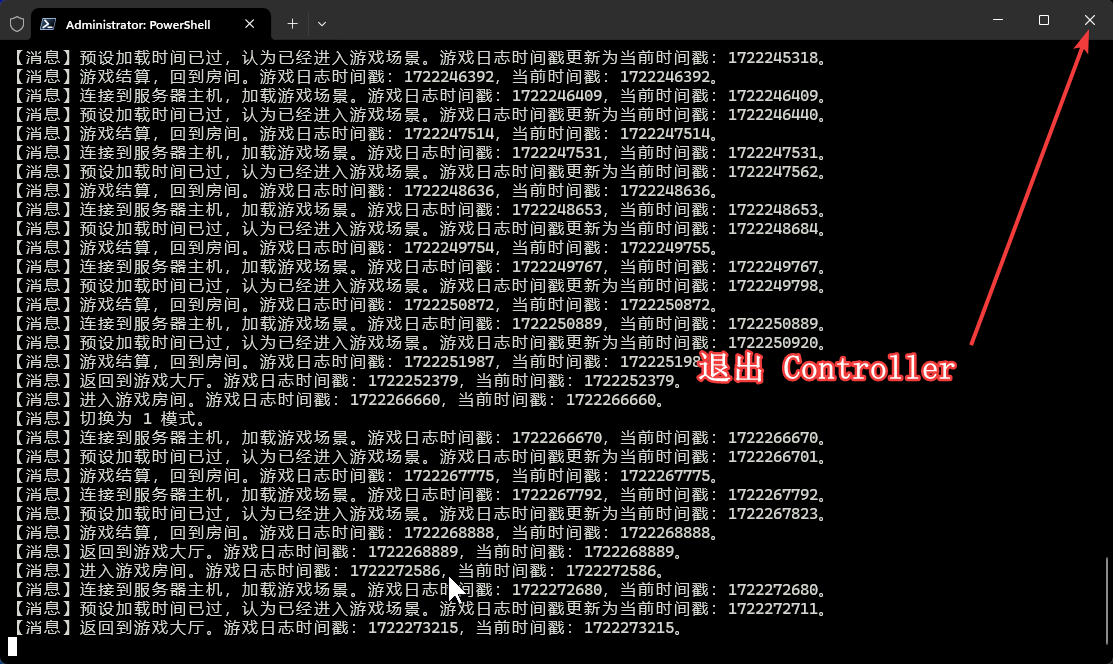
\includegraphics[width=\textwidth]{docs/assets/update/close_controller.png}
    \caption{关闭控制器}
\end{figure}


\begin{figure}[H]
    \Centering
    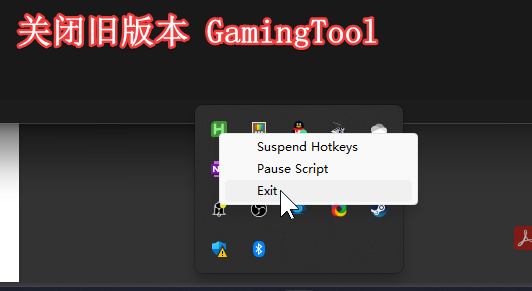
\includegraphics[width=\textwidth]{docs/assets/update/close_gamingtool.png}
    \caption{关闭 \lstinline{GamingTool}}
\end{figure}

下载新版本压缩包。Windows 会将从网络上下载的文件设置为锁定状态,需要在属性中解除锁定。

\begin{figure}[H]
    \Centering
    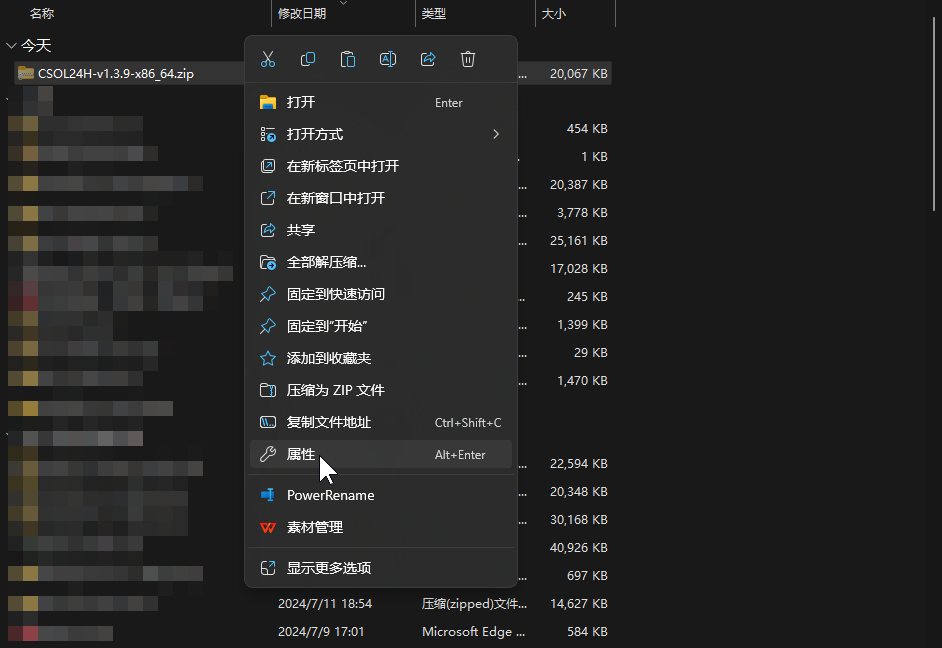
\includegraphics[width=\textwidth]{docs/assets/update/unlock_00.png}
    \caption{点击“属性”}
\end{figure}

\begin{figure}[H]
    \Centering
    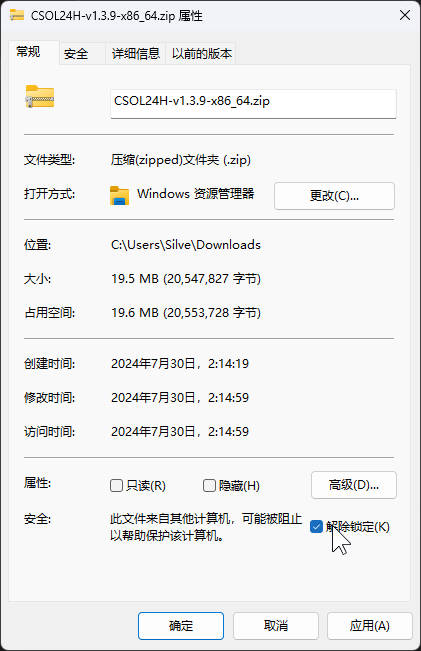
\includegraphics[width=\textwidth]{docs/assets/update/unlock_01.png}
    \caption{解除锁定}
\end{figure}

解压缩新版集成工具。

\begin{figure}[H]
    \Centering
    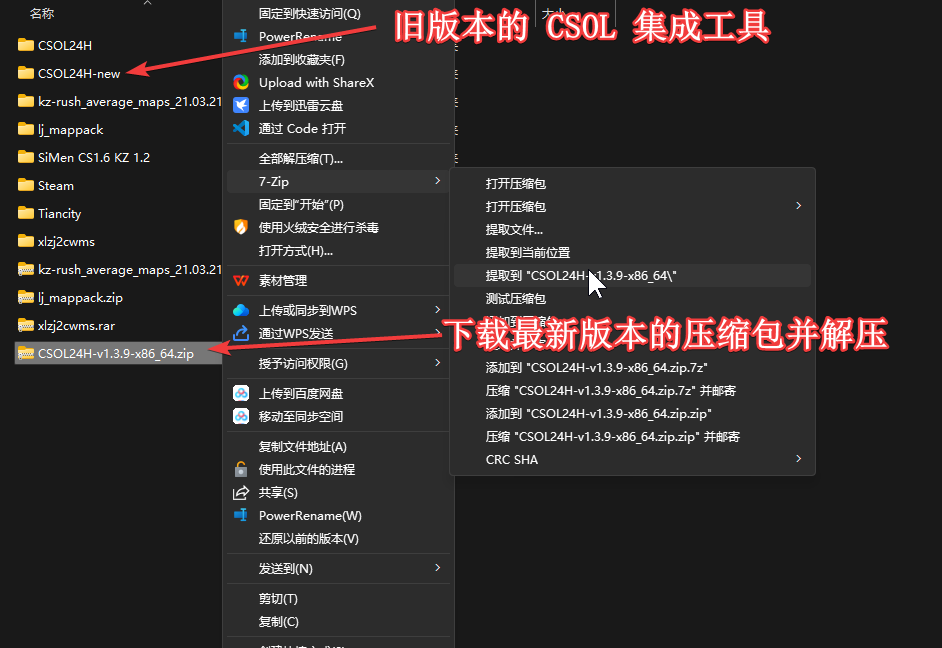
\includegraphics[width=\textwidth]{docs/assets/update/extract_new_version.png}
    \caption{解压新版本压缩包}
\end{figure}

打开您原先使用的旧版本集成工具目录(图中 \lstinline{CSOL24H-new})和解压后的新版本集成工具目录(图中 \lstinline{CSOL24H-v1.3.9-x86_64})。
分别打开 \lstinline{lua} 目录。

\begin{figure}[H]
    \Centering
    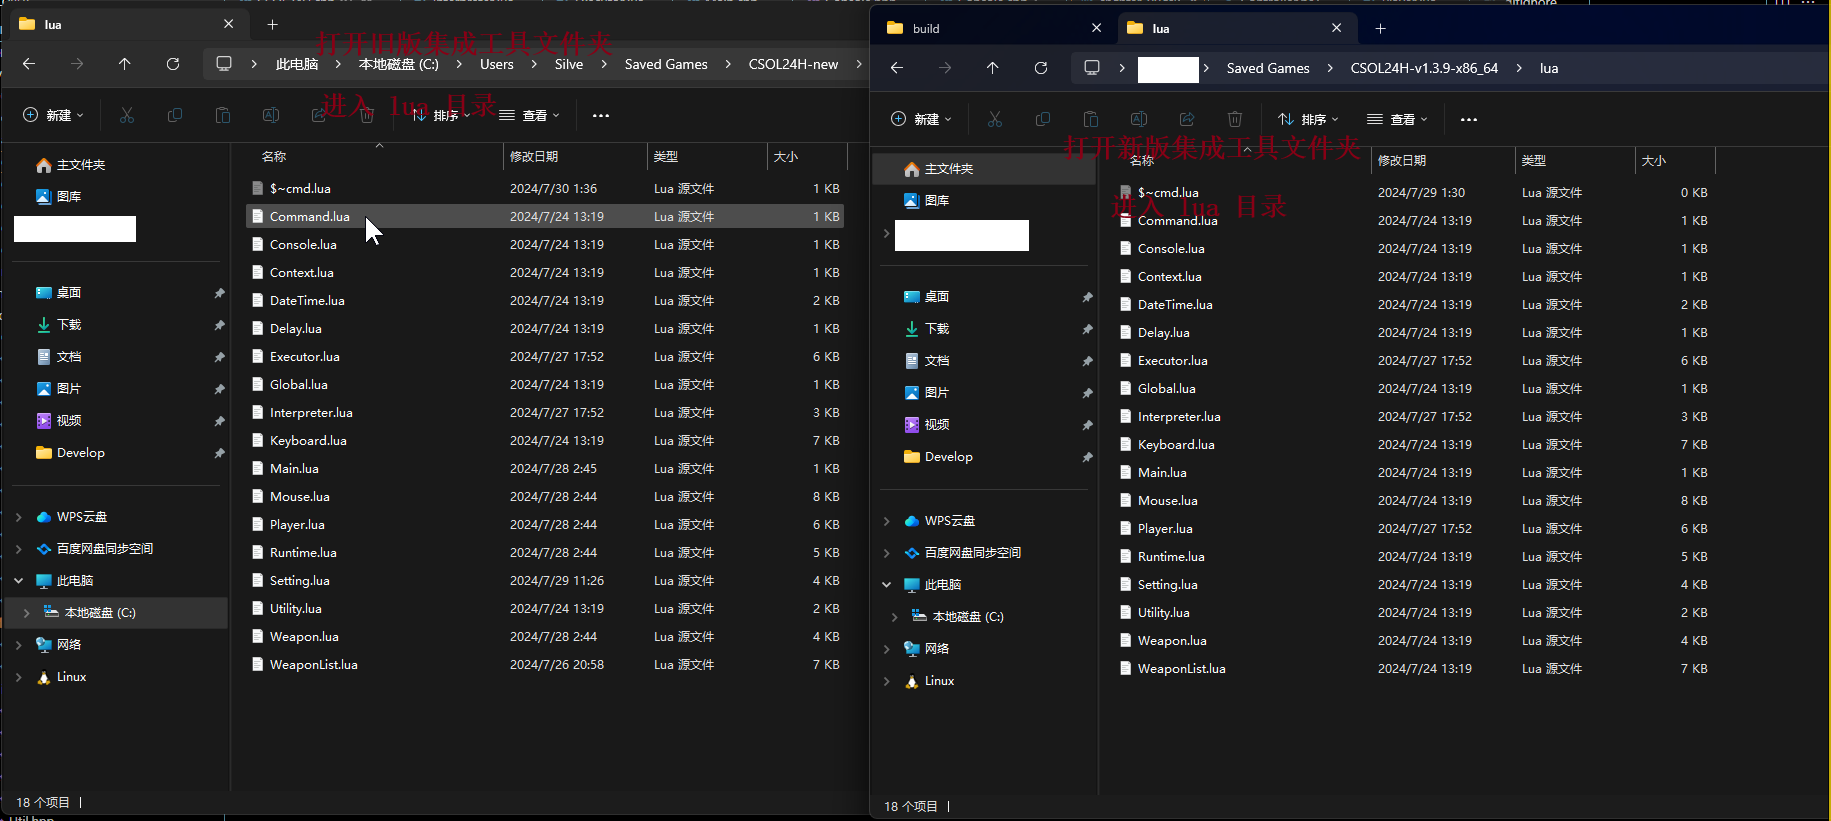
\includegraphics[width=\textwidth]{docs/assets/update/replace_00.png}
    \caption{进入新旧版本集成工具的 \lstinline{lua} 目录}
\end{figure}

然后,按下 \lstinline{Ctrl} 同时选中旧版本集成工具使用的 \lstinline{Setting.lua} 和 \lstinline{WeaponList.lua},然后拖拽到新版本集成工具的 \lstinline{lua} 目录中进行替换。
建议在替换前先查看新版集成工具的配置文件中是否有新增的内容(稳定版本一般不会对配置文件作出更新),若有新增内容,则将其根据您的实际情况添加到您的配置文件中。

\begin{figure}[H]
    \Centering
    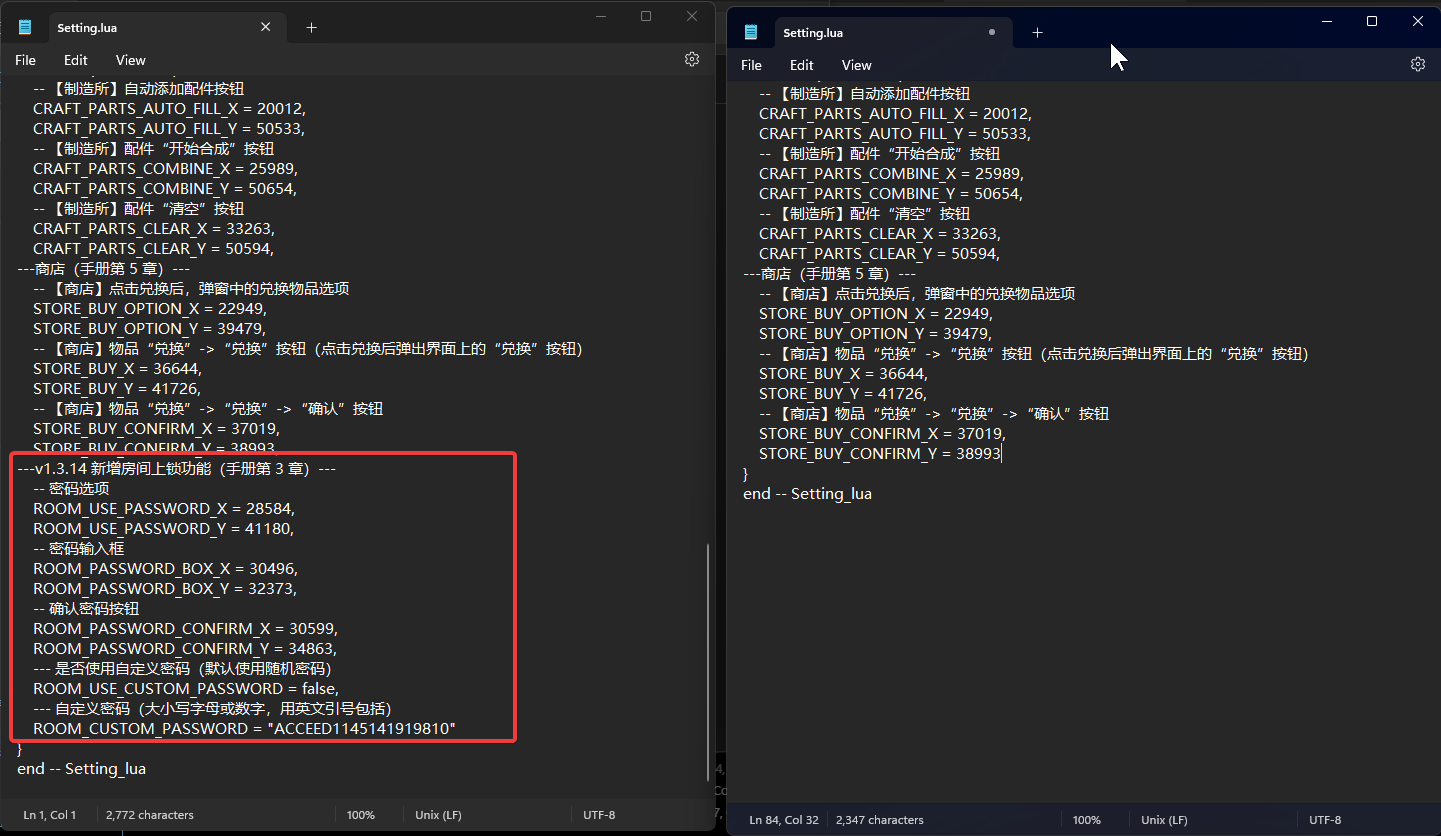
\includegraphics[width=\textwidth]{docs/assets/update/replace_01.png}
    \caption{选中配置文件}
\end{figure}

\begin{figure}[H]
    \Centering
    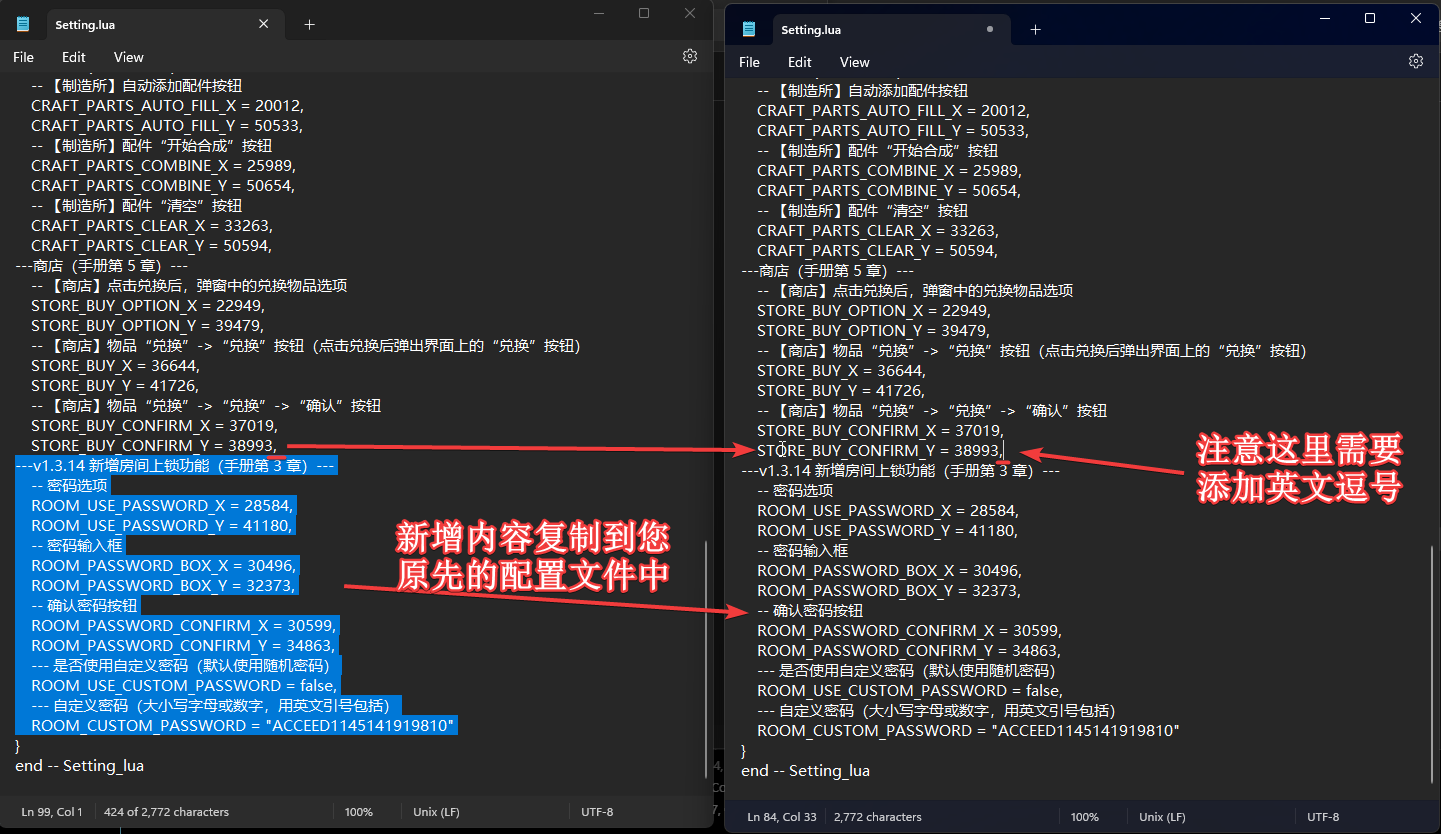
\includegraphics[width=\textwidth]{docs/assets/update/replace_02.png}
    \caption{替换配置文件}
\end{figure}

替换完成后,回到新版集成工具目录下运行 \lstinline{install.ps1},配置新版本集成工具 lua 模块。

\begin{figure}[H]
    \Centering
    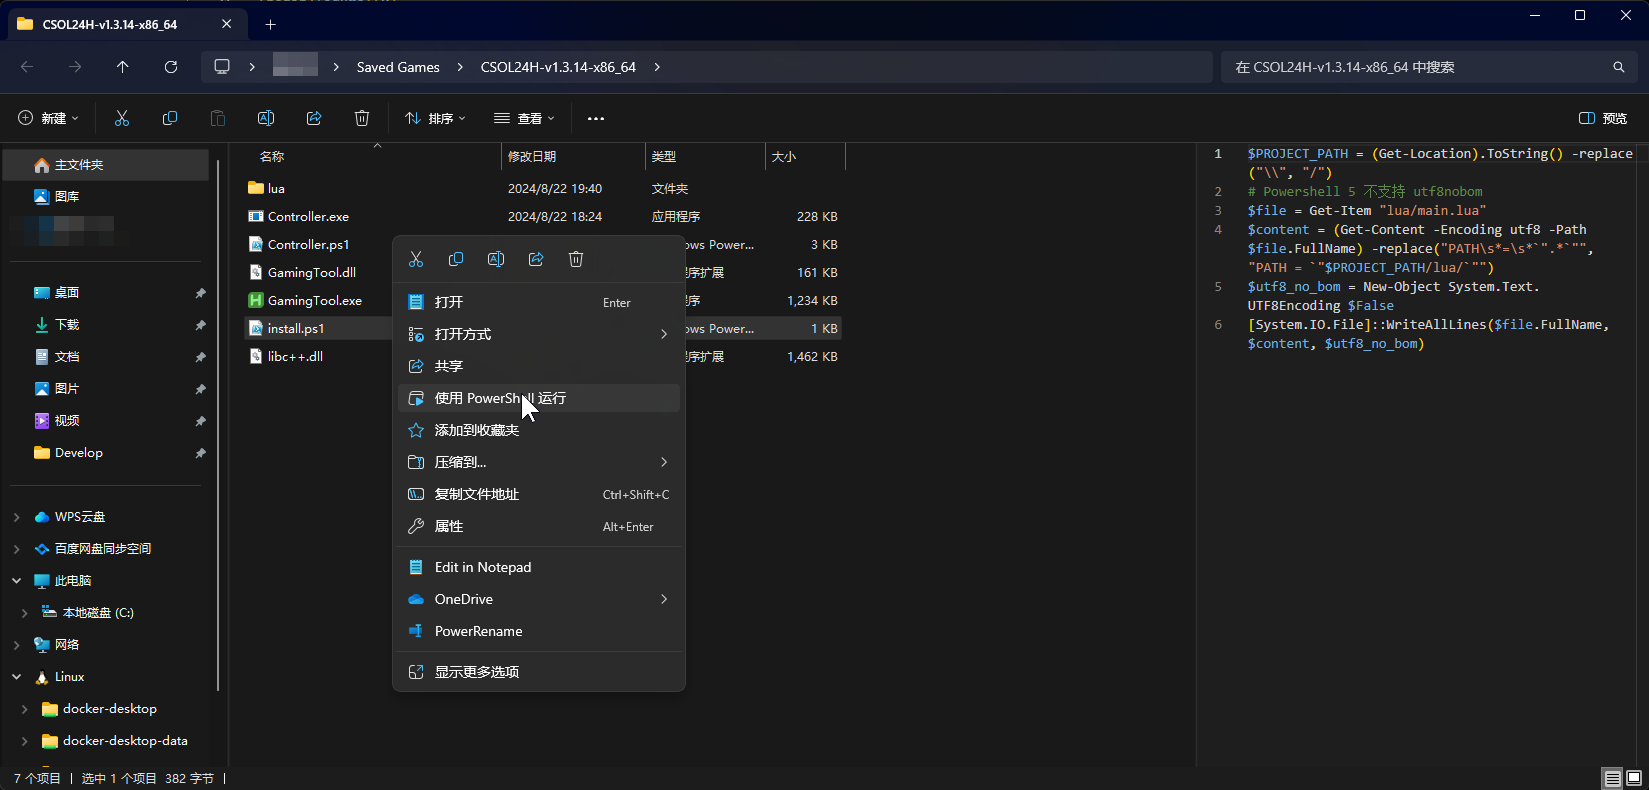
\includegraphics[width=\textwidth]{docs/assets/update/run_install.png}
    \caption{运行 \lstinline{install.ps1}}
\end{figure}

然后,打开罗技软件(确保以管理员权限运行),导入 \lstinline{lua} 目录下的 \lstinline{Main.lua} 文件。

\begin{figure}[H]
    \Centering
    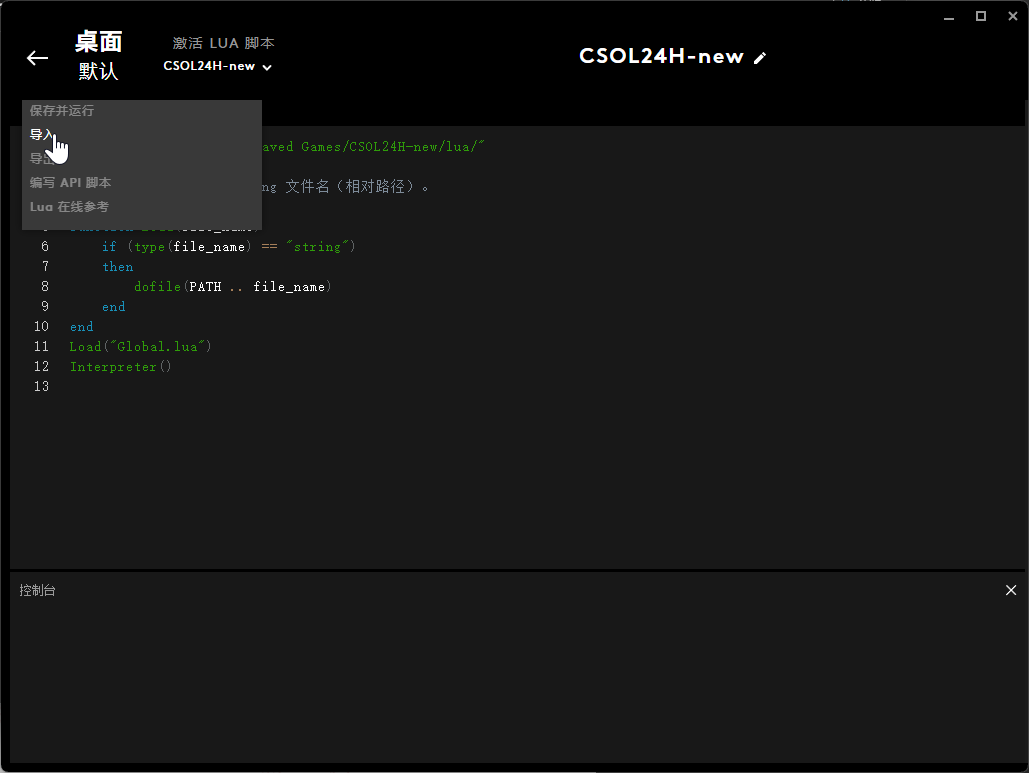
\includegraphics[width=\textwidth]{docs/assets/update/import_main_00.png}
    \caption{点击“导入”}
\end{figure}

\begin{figure}[H]
    \Centering
    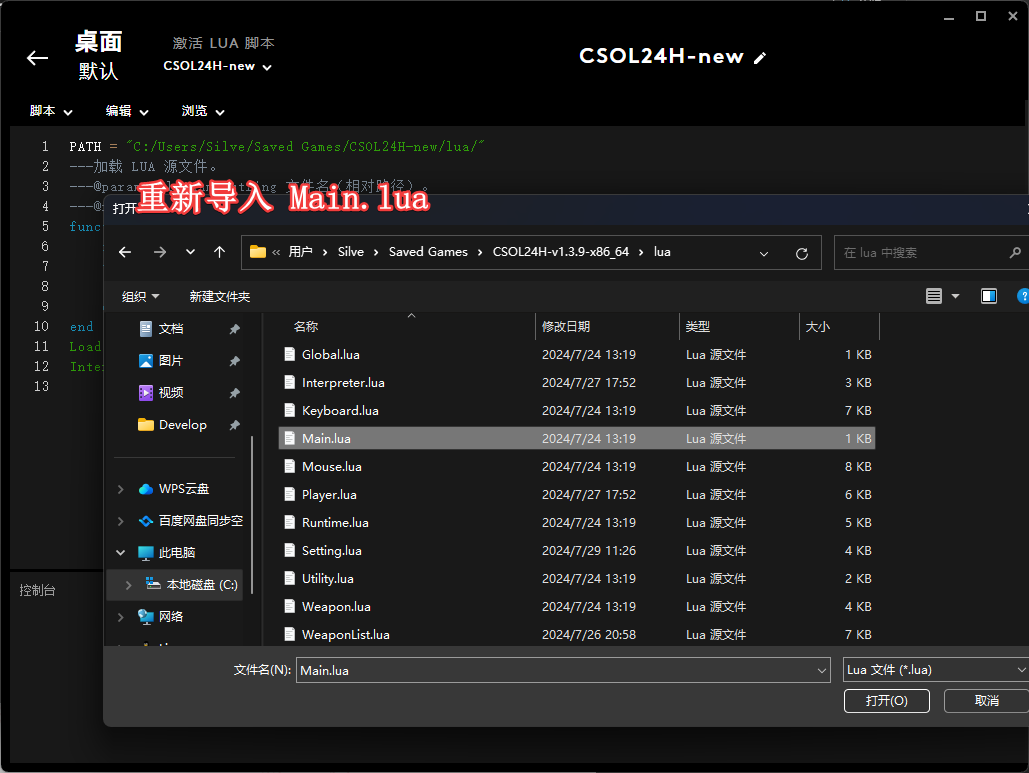
\includegraphics[width=\textwidth]{docs/assets/update/import_main_01.png}
    \caption{导入 \lstinline{Main.lua}}
\end{figure}

然后,保存并运行导入的脚本文件。

\begin{figure}[H]
    \Centering
    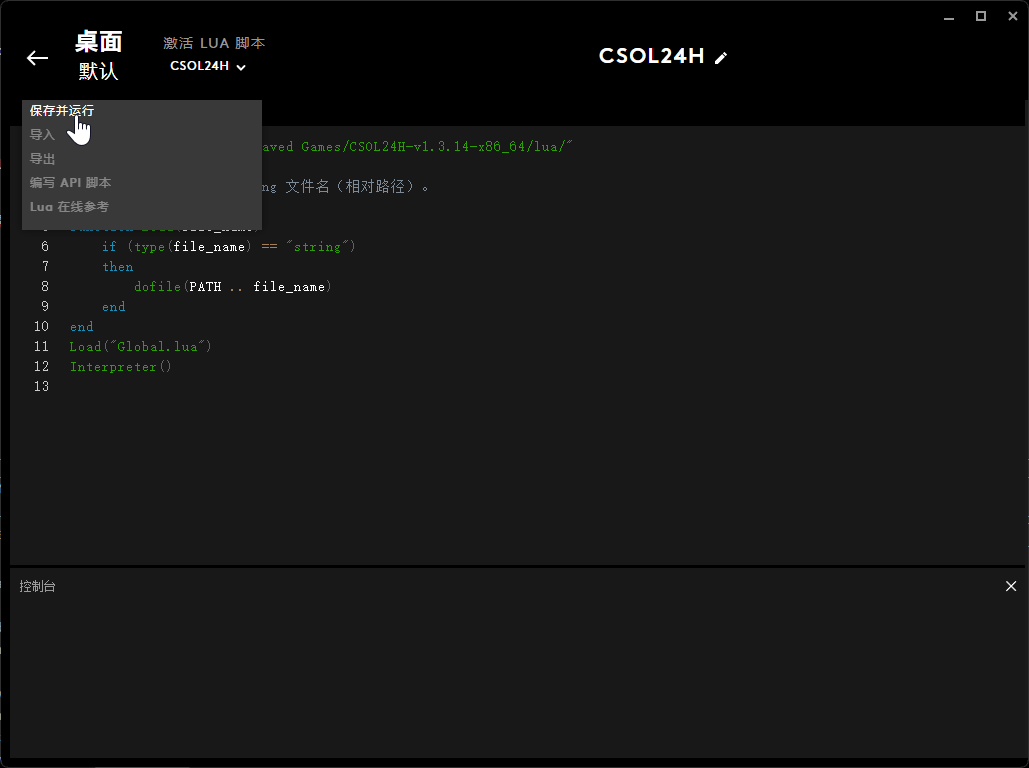
\includegraphics[width=\textwidth]{docs/assets/update/save_and_run_00.png}
    \caption{点击“保存并运行”(也可以按 \lstinline{Ctrl} \lstinline{S} 保存)}
\end{figure}

看到您的配置文件导入信息即表示成功。\textbf{\color{red}当您后续修改配置文件内容时,都需要在此界面中重新导入并保存运行。}

\begin{figure}[H]
    \Centering
    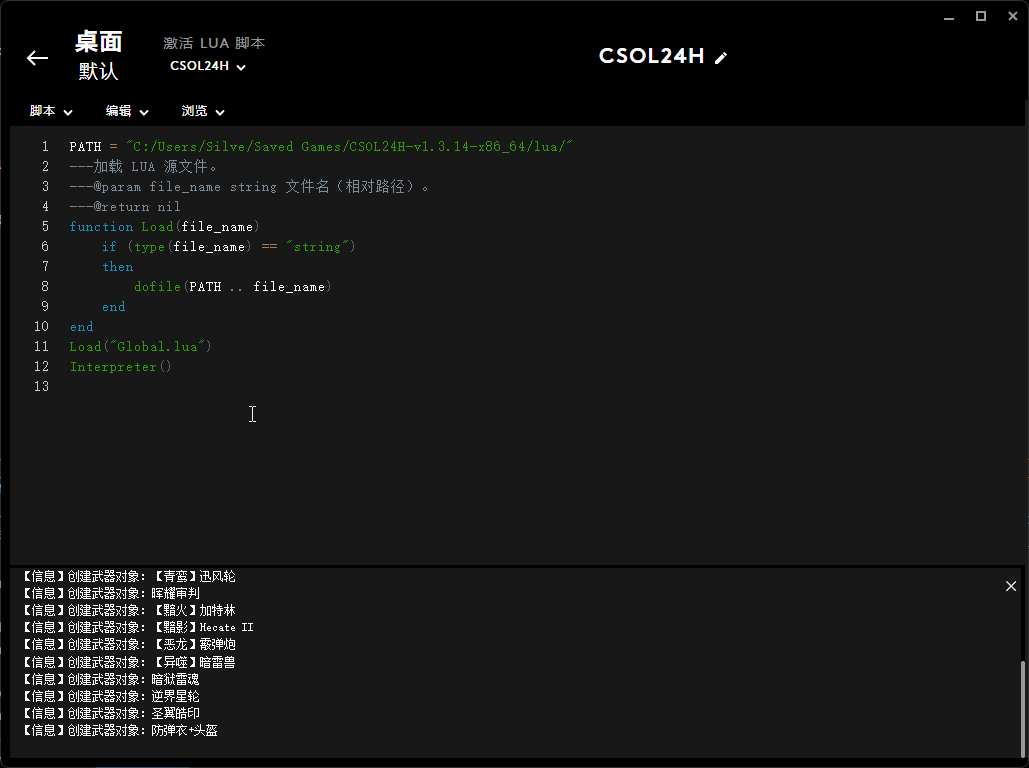
\includegraphics[width=\textwidth]{docs/assets/update/save_and_run_01.png}
    \caption{点击“保存并运行”(也可以按 \lstinline{Ctrl} \lstinline{S} 保存)}
\end{figure}

最后,运行新版集成工具目录下的 \lstinline{GamingTool.exe} 和 \lstinline{Controller.ps1},即可正常使用。

\begin{figure}[H]
    \Centering
    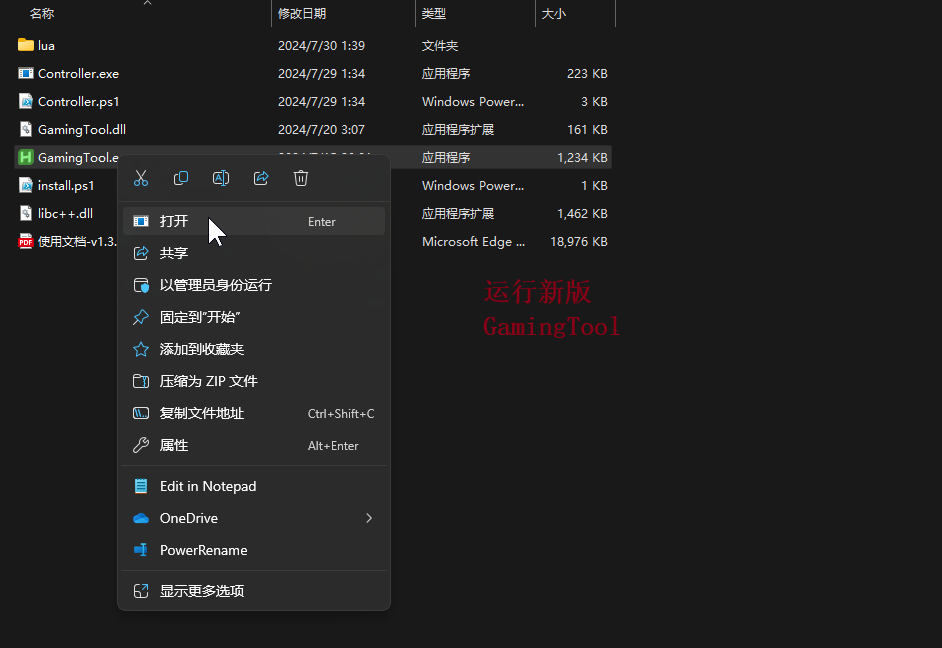
\includegraphics[width=\textwidth]{docs/assets/update/run_new_gamingtool.png}
    \caption{运行 \lstinline{GamingTool}}
\end{figure}

\begin{figure}[H]
    \Centering
    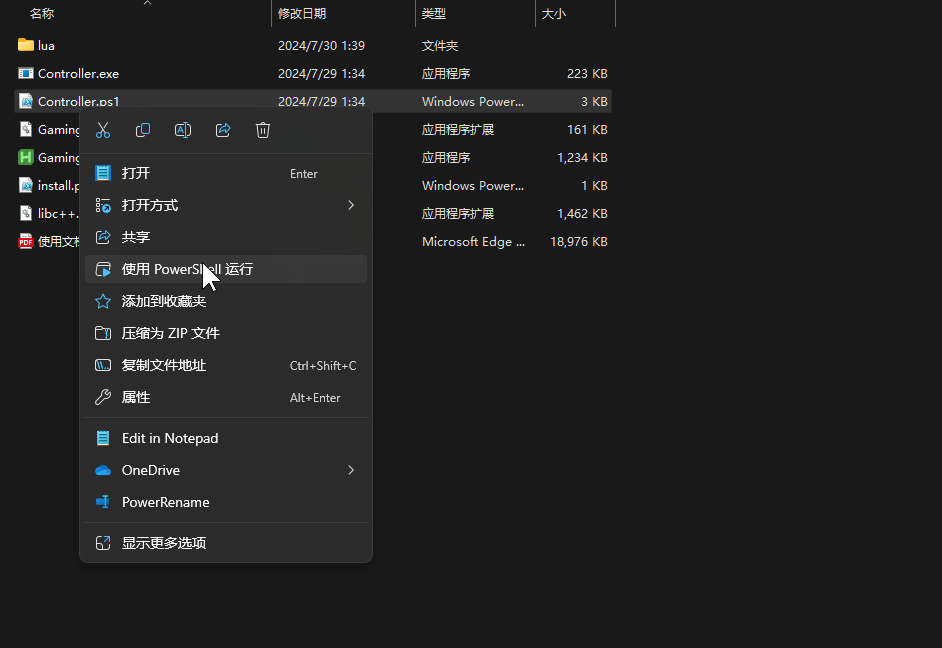
\includegraphics[width=\textwidth]{docs/assets/update/run_new_controller.png}
    \caption{运行 \lstinline{Controller}}
\end{figure}
